% 埼玉大学工学部情報システム工学科
% 卒業論文・修士論文テンプレート
%
% 注意:最新のスタイルファイルは学科Webサイトにて
%       公開されているので、それを必ず確認すること
%
\documentclass[12pt,epsf]{jreport}
\usepackage[dvips]{graphicx} % 図の貼り付け用
\usepackage{ics.utf8} % ICS卒論・修論スタイルファイル
\usepackage{makeidx} %索引生成用パッケージ
\usepackage{tabularx}% 横幅指定で表を作成
\usepackage{latexsym} % 数学記号用パッケージ
\usepackage{url}

\newtheorem{definition}{定義}[chapter]
\newtheorem{algorithm}{アルゴリズム}[chapter]

%% end of local definitions

\def\epsfsize#1#2{\ifnum#1>\hsize\hsize\else#1\fi}

\begin{document}

%論文番号
\papercode{ICS-0XM-XXX} 

% 卒業論文、修士論文のタイトル
\title{卒業論文、修士論文のタイトル} 

%% 所属(学部・学科 or 研究科・専攻・コース)
%\affiliation{工学部情報システム工学科}
%\affiliation{工学部情報工学科}
\affiliation{理工学研究科 数理電子情報系専攻\\情報システム工学コース}

%% 自分の名前。姓と名の間に半角スペースを1ついれること
\author{氏 名}

%% 学籍番号
\studentID{0XYYXXX}

%% 学位論文の提出日
\date{令和3年2月10日提出}

%% 指導教員名(姓名+職位)
\supervisor{○○ ☆☆ 教授}

%% 研究室の所属部署。よくわからないならこのまま
\labaffiliation{埼玉大学 理工学研究科・工学部}

%% 研究室名
\labname{○○研究室}

\maketitle

\setcounter{page}{1}
\chapter*{概要}
 \pagenumbering{roman} % 消さない
 \addcontentsline{toc}{chapter}{概要} %消さない

 概要は,簡潔にまとめること.また,論文の構成も概要の最後に示すこと.


%%% 謝辞 %%%

\chapter*{謝辞}
\addcontentsline{toc}{chapter}{謝辞} % 消さない


研究ならびに生活面においてご指導いただきました○○教授に深く感謝いた
します.

また,先輩としていつもよきアドバイスをくださいました,
○氏,△氏をはじめとする研究室の皆様,そして同期学生の皆様,並びに私
を暖かく見守って頂いた両親はじめとする周囲のすべての皆様に深く感謝いたしま
す.

\tableofcontents % 目次生成
\listoffigures % 図目次生成
\addcontentsline{toc}{chapter}{図目次}
\listoftables % 表目次生成
\addcontentsline{toc}{chapter}{表目次}


\chapter{はじめに} \label{chap:intro}
\pagenumbering{arabic} %消さないこと
\setcounter{page}{1}   %消さないこと

 \section{背景}
 背景


 \section{目的}
 目的


 \section{本論文の構成}
 構成。章や節番号を参照する場合には「\ref{chap:intro}章では…、\ref{chap:exp}章では、\ref{sec:method}節では、」などのように記載する。
 

\chapter{実験} \label{chap:exp}
 \section{実験方法} \label{sec:method}
 実験方法

 \section{実験結果}
 実験結果

 
 \section{図の例}

 基本的には図はページ上部か下部に置くためオプションとしてはtかbを用いる。また、図のキャプション(caption)は図の下に記載する。図の番号は「図\ref{fig:reasoning_engine}」のように参照する。
 
 \begin{figure}[tb]
 \begin{center}
  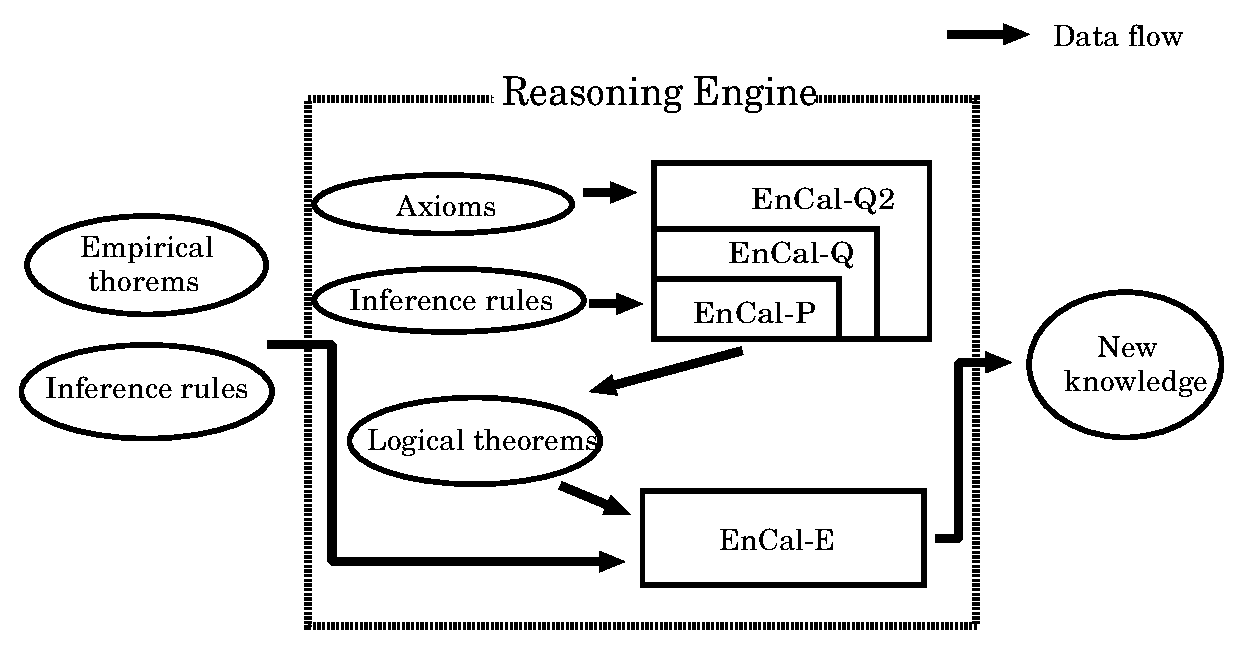
\includegraphics[scale=0.6]{eps/reasoning_engine.eps}
  \caption{The relationship among the parts of EnCal}
  \label{fig:reasoning_engine}
 \end{center}
\end{figure}

 \section{表の例}
 
 基本的には表はページ上部か下部に置くためオプションとしてはtかbを用いる。また、表のキャプション(caption)は表の上に記載する。表の番号は「表\ref{tab:num_of_schemata_satisfied_srp}」のように参照する。

また、表の罫線については誤解を招かないかぎり少なくすることが一般的である。今回の例では、表見出しの下の罫線を2重線にすることで見出しとデータを見やすく分けている。また、縦の罫線は削除している。
 
 \begin{table}[tb]
\begin{center}
\caption{The number of elements of $F_{k}(CML)$ and $FS_{k}(CML)$}
\label{tab:num_of_schemata_satisfied_srp}
 \begin{tabular}{c l l}
  \hline
 degree & $F_{k}(CML)$ &$FS_{k}(CML)$ \\
    & (a)&  (b)\\ 
  \hline
  \hline
  1 &  $1.60 \times 10^{1}$ & $4.00 \times 10^{0}$\\
  2 & $2.26 \times 10^{3}$ & $2.60 \times 10^{2}$  \\
  3 & $1.67 \times 10^{8}$ & $8.90 \times 10^{6}$\\
  4 & $2.92 \times 10^{19}$ & $5.15 \times 10^{17}$\\
  5 & $1.63 \times 10^{45}$ & $6.31 \times 10^{42}$\\
  6 & $4.29 \times 10^{103}$ & $2.13 \times 10^{100}$\\
  7 & $1.02 \times 10^{235}$ & $3.09 \times 10^{230}$\\
  8 & $8.15 \times 10^{527}$ & $5.61 \times 10^{521}$\\ 
  \hline
 \end{tabular}
\end{center}
\end{table}




\chapter{考察}
考察

\chapter{おわりに}
 \section{まとめ}
 まとめ

 \section{今後の課題}
 今後の課題


%%% 修士論文の場合は必須。卒業論文の場合は任意
\chapter*{公表論文}
\addcontentsline{toc}{chapter}{公表論文}

\begin{list}%
 {} %default label
 {} %formatting parameter
 \item 査読付き論文
       \begin{itemize}
	\item Hogehoge: ....
       \end{itemize}
 \item 査読なし論文
       \begin{itemize}
	\item Hogehoge: ....
       \end{itemize}
\end{list}
%%% 修士論文必須ここまで %%%

\newpage

% 参考文献:bibtexを使う場合
%
%\bibliographystyle{BSTファイル名} % bstファイル名
%\bibliography{refs} % bibファイル名

% 参考文献:直接記述する場合
\begin{thebibliography}{99}
\label{sannkoubunnkenn_chapter}

%% 参考文献形式例
%
% ここには媒体別に並べているが普通は、
% 第一著者の姓の頭文字でアルファベット順(A - Z、あ〜ん)あるいは、
% 引用順に並べること。どちらにするかは指導教員に確認すること。

% 先端情報システム工学研究室における学位論文の参考文献形式
% http://www.aise.ics.saitama-u.ac.jp/~gotoh/FormatOfReferencesInAiseLab.html

% 学術雑誌論文
% 著者名: 論文題目, 学術雑誌名, 巻, 号, ページ数, (出版社 or 出版団体), 発表年月.
\bibitem{tagawa98}
多川 孝央, 大堀 順也, 程 京徳, 牛島 和夫: 相関論理における強相関性原理,
        人工知能学会誌, Vol.\ 13, No. 3, pp.\ 387-394, 1998年5月.

\bibitem{Nonaka99}
Yusuke Nonaka, Jingde Cheng, and Kazuo Ushijima: A Tasking Deadlock
        Detector for Ada 95 Programs, Ada User Journal, Vol.\ 20, No.\ 1,
        pp.\ 79-92, April 1999.

% 電子出版のためページ数が割り振られてなく、記事番号1222が割り振られている例。
\bibitem{Sa2016}
        Inkyu Sa, Zongyuan Ge, Feras Dayoub, Ben Upcroft, Tristan Perez, and Chris McCool: DeepFruits: A Fruit Detection System Using Deep Neural Networks, Sensors Vol.\ 16 No.\ 8, e1222, August 2016.

        
% 単行本
%  著者名(編集者、訳者): 書名, 出版社 or 出版団体, 発表年月.
\bibitem{ChengXX}
程 京徳: 相関論理入門, 何らか出版社, 200?年?月.

\bibitem{Jin01}
Qun Jin, Jie LI, Nan Zhang, Jingde Cheng, Clement Yu, and Shoichi
        Noguchi: Enabling Society with Information Technology,
        Springer-Verlag, November 2001.

% 翻訳本の場合は原著の情報の後に翻訳本の情報を書く
\bibitem{Hennessy93}
Matthew Hennessy: The Semantics of Programming Languages, John Wiley and
Sons, Ltd., 1990. (マシュー ヘネシー著, 荒木 啓二郎, 程 京徳 共訳: プロ
グラミング言語の意味論入門, サイエンス社, 1993年.)

% 国際会議、国内シンポジウム論文集論文
% 著者名: 論文題目, 会議名+会議略称, ページ数, 会議開催地, 会議開催国,(出版社 or 出版団体), 発表年月.
\bibitem{Goto01}
Yuichi Goto, Daisuke Takahashi, and Jingde Cheng: Parallel Forward
        Deduction Algorithms of General-Purpose Entailment Calculus on
        Shared-Memory Parallel Computers, Proceedings of the ACIS 2nd
        International Conference on Software Engineering, Artificial
        Intelligence, Networking \& Parallel/Distributed Computing,
        pp.\ 168-175, Nagoya, Japan, August 2001.

\bibitem{Koide01}
小出 雅人, 程 京徳: インターネット上でカードゲームを行うための汎用プロト
        コル群の開発, 情報処理学会第6回ゲーム・プログラミング国際ワーク
        ショップ論文集, pp.\ 78-85, 箱根, 日本, 2001 年10月.

% 論文集シリーズや単行本に収録された論文
% 著者名: 論文題目, 編集者(editor), 書名, 論文集シリーズ名, 論文集シリーズ巻数, ページ数, 出版社 or 出版団体, 発表年月.
\bibitem{Cheng91}
Jingde Cheng: Relevance Logic and Entailment Logic, in I.\ Nakada and
        M.\ Hagiya (Eds.), ``Software Science and Engineering,''
        pp.\ 189-211, World Scientific, November 1991.

\bibitem{Nonaka00}
Yusuke Nonaka, Jingde Cheng, and Kazuo Ushijima: A Supporting Tool for
        Development of Self-measurement Ada Programs, in H.\ B.\ Keller
        and E.\ Ploedereder (Eds.), ``Reliable Software Technologies -
        Ada-Europe 2000, 5th International Conference on Reliable
        Software Technologies, Potsdam, Germany, June 2000,
        Proceedings,'' Lecture Notes in Computer Science, Vol.\ 1845,
        pp.\ 69-81, Springer-Verlag, June 2000.


% 博士,修士,卒業論文
\bibitem{Goto05}
後藤 祐一: 強相関論理に基づいた自動前向き演繹とその応用, 埼玉大学大学院
	理工学研究科情報数理科学専攻博士論文, 2005年3月.

\bibitem{Goto02}
後藤 祐一: 強相関論理と汎用前向き自動帰結演算システム EnCal を用いた知識
	発見, 埼玉大学大学院理工学研究科情報システム工学専攻修士論文, 2003年
	2月.

\bibitem{Goto00}
後藤 祐一: 汎用前向き自動帰結演算システムEnCalの共有メモリ型並列計算機上
	での並列化, 埼玉大学工学部情報システム工学科卒業論文, 2001年2月.


% 企業や製品のWebページなど
% \newblockは後ろに続く文字列を一つの塊としてみなす命令
\bibitem{cem}
Common Criteria Project: CEM v3.1,
\url{http://www.commoncriteriaportal.org/thecc.html}
(accessed 2007-04-05).

\bibitem{ipsjweb}
情報処理学会: コンピュータ博物館設立の提言, \url{http://www.ipsj.or.jp/03somu/teigen/museum200702.html} (参照2007-02-05).

\end{thebibliography}

% 付録
\appendix % 以下,付録
\chapter{▽△▽△}
\section{ほげほげ}
\section{ほりゃほりゃ}
\chapter{▽△▽△}
\section{ほげほげ}
\section{ほりゃほりゃ}

% 索引をつける場合には
% mendexかmkindexで作成
%\printindex

%目次にIndexを表示させる場合はmendexかmkindex実行後に作成される
% hogehoge.idmファイルのtheindex環境の中で下記命令を置く
%\addcontentsline{toc}{chapter}{Index}

\end{document}

